% ****** Start of file apssamp.tex ******
%
%   This file is part of the APS files in the REVTeX 4.1 distribution.
%   Version 4.1r of REVTeX, August 2010
%
%   Copyright (c) 2009, 2010 The American Physical Society.
%
%   See the REVTeX 4 README file for restrictions and more information.
%
% TeX'ing this file requires that you have AMS-LaTeX 2.0 installed
% as well as the rest of the prerequisites for REVTeX 4.1
%
% See the REVTeX 4 README file
% It also requires running BibTeX. The commands are as follows:
%
%  1)  latex apssamp.tex
%  2)  bibtex apssamp
%  3)  latex apssamp.tex
%  4)  latex apssamp.tex
%
\documentclass{article}
\usepackage{graphicx}% Include figure files
\usepackage{dcolumn}% Align table columns on decimal point
\usepackage{bm}% bold math
\usepackage{booktabs}
\usepackage{listings}
\usepackage{listing}
\usepackage{color}
\usepackage{hyperref}
\usepackage{url}
\usepackage{subfig}
\usepackage{parcolumns}
\usepackage{amsmath}
\usepackage{cite}
\usepackage{blindtext}
\usepackage[utf8]{inputenc}
%\usepackage{tocloft}
%\usepackage{hyperref}% add hypertext capabilities
%\usepackage[mathlines]{lineno}% Enable numbering of text and display math
%\linenumbers\relax % Commence numbering lines

%\usepackage[showframe,%Uncomment any one of the following lines to test
%%scale=0.7, marginratio={1:1, 2:3}, ignoreall,% default settings
%%text={7in,10in},centering,
%%margin=1.5in,
%%total={6.5in,8.75in}, top=1.2in, left=0.9in, includefoot,
%%height=10in,a5paper,hmargin={3cm,0.8in},
%]{geometry}

\definecolor{codegreen}{rgb}{0,0.6,0}
\definecolor{codegray}{rgb}{0.5,0.5,0.5}
\definecolor{codepurple}{rgb}{0.58,0,0.82}
\definecolor{backcolour}{rgb}{0.95,0.95,0.92}

\lstdefinestyle{mystyle}{
    backgroundcolor=\color{backcolour},
    commentstyle=\color{codegreen},
    keywordstyle=\color{magenta},
    numberstyle=\tiny\color{codegray},
    stringstyle=\color{codepurple},
    basicstyle=\footnotesize,
    breakatwhitespace=false,
    breaklines=true,
    captionpos=b,
    keepspaces=true,
    numbers=left,
    numbersep=5pt,
    showspaces=false,
    showstringspaces=false,
    showtabs=false,
    tabsize=2
}

\lstset{style=mystyle}
\begin{document}
	\renewcommand*{\lstlistlistingname}{List of Code}
	\renewcommand*\lstlistingname {Listing}
	%\preprint{APS/123-QED}

	\title{Optical Coherence Tomography: \\ Mitigation of Scattering Using DSP Techniques}

	\author{Jared Mann, V00187636}
	\author{Mike Vlanich, V00862757}
	\author{University of Victoria, Faculty of Electrical Engineering}

	\date{\today}% It is always \today, today,


	\begin{abstract}
Optical Coherence Tomography (OCT) is a non-invasive method of producing 2-Dimensional images of biological tissues. The practice came into prominence in 1991 from the developments of Huang et al. Since its introduction advancements in laser diode technology and imagery has allowed for micrometer resolution and is widely used in the Ophthalmology.\cite{bhende_optical_2018} Although OCT produces great resolution there are drawbacks. OCT is notorious for producing a phenomenon called ‘speckle noise’. This review will utilize previous work done using imagery filters to reduce speckle noise and as well create our own simulations to confer.
	\end{abstract}

	%\pacs{Valid PACS appear here}% PACS, the Physics and Astronomy
	% Classification Scheme.
	%\keywords{Suggested keywords}%Use showkeys class option if keyword
	%display desired
	\maketitle
	\tableofcontents
	\makeatletter
	\let\toc@pre\relax
	\let\toc@post\relax
	\makeatother

  	\listoffigures
  	\listoftables


  	\lstlistoflistings
  	%\makeatletter

  	%\print@toc {lol}
  	%\makeatother

	\section{Introduction}

	Optical Coherence Tomography (OCT) is a non-invasive method of producing 2-Dimensional images of internal tissues in a method comparable to that of ultrasound imaging.\cite{Huang91}\cite{sander_optical_2011} The practice came into prominence following the developments of Huang et al. at the Massachusetts Institute of Technology in 1991. \cite{Huang91}




	\section{\label{sec:level1}OCT Identified Problem and Suggested Solution}
	\subsection{\label{sec:level2} The Problem of Speckle Noise}
	\begin{figure}
		\centering
		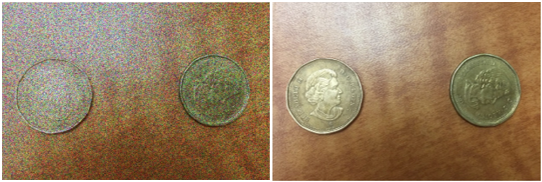
\includegraphics[width=0.7\linewidth]{Figures/specklefilter2}
		\caption{On the left is an image put through a speckle filter in Matlab. On the right is the original image.}
		\label{fig:specklefilter2}
	\end{figure}
	A problem with using an OCT interferometer is that ‘speckle’ noise exists, which ultimately reduces the quality of the image. Speckle is a phenomenon that is caused by interference of the reflected wave at the photo-detector. Speckle noise is evident when trying to image non-fluid structures (such as hard tissue). As the wave propagates it becomes distorted due to “low-angle multiple forward scattering and diffuse multiple backscattering of coherent photons”. \cite{Popescu2007}

	In OCT interferometry imaging, photons are detected after one backscattering event for most relevant information, but when a wave is propagated through a dense biological sample it experiences numerous scattering events (in OCT interferometry). These scattering events increase the likelihood for photons to change their travel distance comparative to their airborne path which results in speckle noise reducing the image quality. \cite{Popescu2007}

	To display the effects of speckling on an image refer to Figure \ref{fig:specklefilter2}. Using $imnoise(I,'speckle',v)$ in Matlab to create a filter that would add multiplicative noise to an image. As seen on the left the image resolution is decreased significantly after adding speckling noise especially in the area of high light reflectivity off of the table.

	\subsection{\label{sec:level2} Possible Solutions for Speckle Noise}
	As technology progress in imaging processing, techniques are being developed to help reduces the effects of speckle noise when using OCT. Some of these methods include decreasing spatial and temporal coherence of the laser used. While more trivial techniques such as phase-domain processing and zero-adjustments are used to improve image quality due to speckle noise. \cite{Popescu2007}

	\section{\label{sec:level1} OCT Image Aquisition and Preparation}

	\subsection{\label{sec:level2} Aquiring and Visualizing OCT Images}
		While many published reports contain printed images of OCT captures, getting raw data was necessary to make realistic observations on the effects of using digital filtering. 3D OCT captures of healthy individuals were obtained from a publised proceeding comparing OCT scans of healthy individuals \cite{tahereh_2014}. The scans were provided in .mat file format. The size of each volume provided by these scans was 650 x 512 x 128 voxels. Each voxel had a resolution of 11.72 x 46.88 x 3.54 $\mu$m. We were able to view an interactive 3D volume from the provided .mat files using a script published on MathWorks file exchange titled \textit{3D Volume Visualization} \cite{stough}. A capture of the visualizan can be seen in Figure \ref{fig:3dvol}.



	\subsection{\label{sec:level2} Slicing and Preparing a 2D Image for Processing}
		Upon importing the .mat files into Matlab, they took the form of a 650 x 512 x 128 double data type named d3. The Matlab code shown in Listing \ref{code:2dslicecode} shows the process of taking the middle XY slice and creating a greyscale image.
		\begin{lstlisting}[language=Matlab, caption=Take Slice of 3D Volume, label=code:2dslicecode]
	%Take Slice of 3D Volume
	SliceL = d3(:,:,64);
	ImgSliceL = mat2gray(SliceL, [0 255]);
	imshow(ImgSliceL);
		\end{lstlisting}
		\begin{figure}
			\centering
			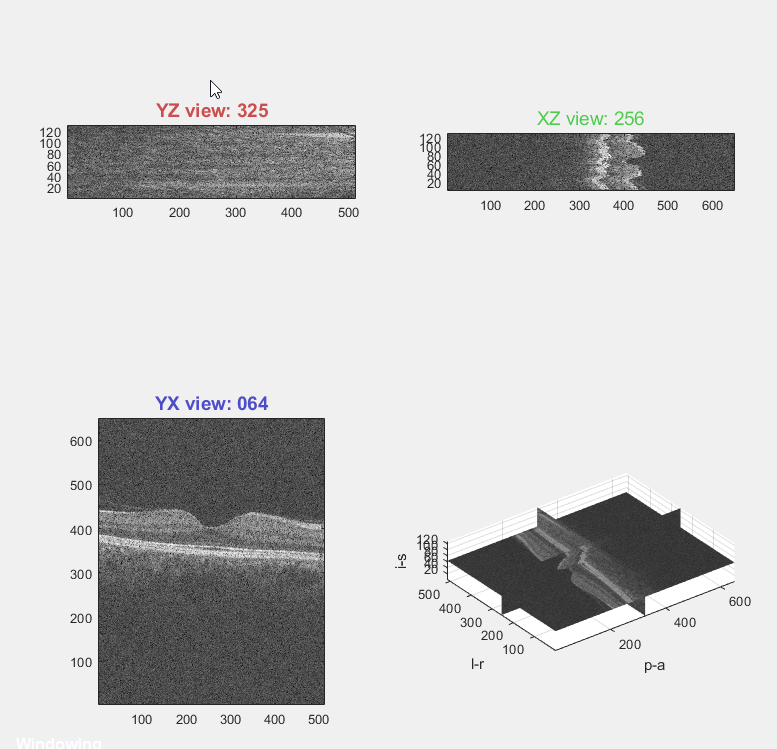
\includegraphics[width=0.7\linewidth]{Figures/3dvol}
			\caption{3D Volume Visualization Capture}
			\label{fig:3dvol}
		\end{figure}
		An example unaltered aquired image is shown in Figure \ref{fig:2dslice}.
		\begin{figure}
			\centering
			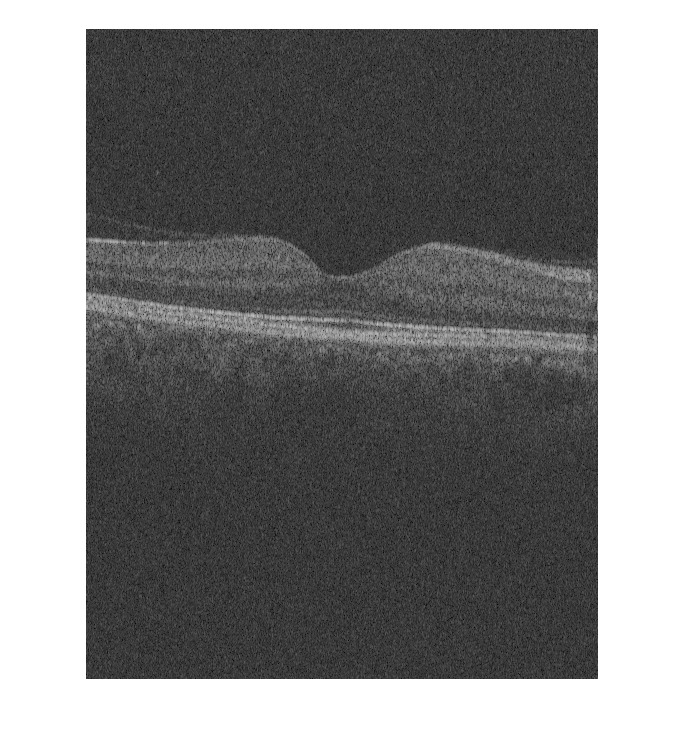
\includegraphics[width=0.7\linewidth]{Figures/2dslice}
			\caption{Unaltered 2D Slice of 3D Volume}
			\label{fig:2dslice}
		\end{figure}

	\section{\label{sec:level1} Quality Metrics: Signal to Noise Level, and Estimated Noise Level}
	The results of quality measurements for each applied filter method are listed in Table (**ADD REFERENCE TO TABLE). The methods for obtaining the quality metrics are described in the following paragraphs.

	\subsection{\label{sec:level2} Contrast to Noise (CNR) Estimation}
	The code shown in Listing \ref{code:cnr} outlines the process for aquiring the contrast to noise estimation. The process starts with taking the 2D image matrix and converting it into a 1D array.

	The maximum and minimum values are extracted from the 1D matrix, and then the standard deviation is calculated. The final CNR is calculated equivalent to the formula:

	$$CNR = (\frac{Max-Min}{\text{Standard Deviation}})$$

	\begin{lstlisting}[language=Matlab, caption=Estimate Contrast to Noise Ratio, label=code:cnr]
	% Measure contrast-to-noise ratio
	img=ImgSliceL;
	img=double(img(:));
	ima=max(img(:));
	imi=min(img(:));
	mse=std(img(:));
	cnr=((ima-imi)./mse)
	\end{lstlisting}

	\subsection{\label{sec:level2} Estimated Noise Level}
	The Estimated Noise Level (ENL) is calculated using a method implemented in a Matlab function by Ashish Meshram \cite{meshram_noise_2014}. This implementation is based off of the paper titled \textit{Single-Image Noise Level Estimation for Blind Denoising}  by Xinhao Liu, and team \cite{Liu_2013}.
	\subsection{\label{sec:level2} Naturalness Image Quality Evaluator (NIQE) No-Reference Image Quality Score}

	Due to the fact that all obtained images need to be evaluated as is, with no reference image to compare to, it is advantageous to use a metric that does not require a reference image. Matlab has a built-in function called niqe that returns a value (lower is better, indicating higher perceptual quality) using the Naturalness Image Quality Evaluator based off the work of Anish Mittal and team \cite{NIQE_2013}.
  \subsection{\label{sec:level2} Omission of Mean Squared Error (MSE) for OCT Images}

  In the analysis of filter quality, a metric called Mean Squared Error (MSE) is often used to compare an image without any distortion to an image that has been distorted and then filtered. In our analysis we do not have the ability to do this, because we have an image that has distortion inherent in its aquisition.

  In the paper titled \textit{Speckle reduction in optical coherence tomography images using digital filtering} \cite{ozcan_speckle_2007} the reference image used for calculating the MSE of filters was a composite image made from using multiple scans see Figure \ref{fig:composite} for the reference image used in the paper (where N=64). In these images the N value represents the number of scans used to make the composite.

  \begin{figure*}
    \centering
    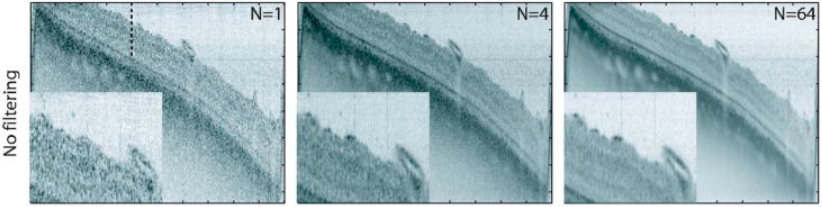
\includegraphics[width=0.7\linewidth]{Figures/composite}
    \caption{OCT Captures with Increasing Numbers of Composite Images Used, Adapted From \cite{ozcan_speckle_2007}}
    \label{fig:Composite}
  \end{figure*}

  Since we do not have access to a composite image, or an image without inherent distortion, an MSE evaluation of filtering will be omitted from our report.
	\section{\label{sec:level1} Scope of DSP Methods Used}

	This report will focus on 2D image filtering methods which can be applied using Matlab, and due to our resources we will not be able to make composite captures from multiple scans.

	\subsection{\label{sec:level2} Wiener Filter}
	The 2D Wiener filter is a processing technique which is capable of not only improving resolution but as well signal-to-noise (SNR) ratio of particular image. This low-pass filter is an optimal trade-off between inverse filtering and noise smoothing. This filter is also referred to as a local linear minimum mean square error which means [LLMMSE] it is the optimal estimator in the sense of mean squared error (MSE). Where LLMMSE and MSE is determined by:
$$
\begin{bmatrix}
R_{xx}[0] & R_{xx}[-1] & ... & R_{xx}[1-N]\\
R_{xx}[1] & R_{xx}[0] & ... & R_{xx}[2-N]\\
\vdots & \vdots & \ddots & \vdots \\
R_{xx}[N-1] & R_{xx}[N-2] & ... & R_{xx}[0]
\end{bmatrix}
\begin{bmatrix}
h[0]\\
h[1]\\
\vdots\\
h[N-1]
\end{bmatrix}
$$
$$
=
\begin{bmatrix}
R_{yx}[0]\\
R_{yx}[1]\\
\vdots\\
R_{yx}[N-1]
\end{bmatrix}
$$

$$R_{ee}[m]=R_{yy}[m]-R_{yy}[m] = R_{yy}[m]-h[m] \times R_{xy}[m]$$

Where $R_{xx}$ is the received signal, N is the length, then there are N equations in the N unrestricted values of h[n] and h[m] is the impulse response of the filter \cite{Oppenheim_2015}. Refer to Figure \ref{fig:unfiltwienerfilt} for the resulting image.


\subsection{\label{sec:level2} Lee Filter}
The Lee filter applies a spatial filter to each pixel which filters data based on local statistics calculated within a square window. The value of the center pixel is replaced by a value calculated using the neighbouring pixels. Implements similar characteristics of the Wiener filter in the sense it uses MSE but also has edge preserving features \cite{leefilter}. The pixels are classified into:
\\
Homogenous: where the pixel value is replaced by an average of the filter window
\\
Heterogenous: where the pixel value is replaced by a weighted average
\\
Point: where the pixel value is unchanged.
\\
\\
The resultant gray value R for the pixels is then represented as:
$$R = I_{m} \text{ for } C_{i} \leq C_{u}$$
$$R = I_{m} \times W+I_{c} \times (1-W) \text{ for } C_{u}<C_{i}<C_{max}$$
$$R = I_{c} \text{ for } C_{i} \geq C_{max}$$

Where:
\\
	$I_{m}$ = mean value of intensity within the kernel
	\\
	$I_{c}$ = center pixel in the kernel
	\\
	$C_{i}$ = S/$I_{m}$
	\\
	$C_{u}$ = $\sqrt{1/(number of locks)}$
	\\
	W				= $\exp{-\zeta(C_{i}-C_{u})/(C_{max}-C_{i})}$
	\\
	S       = standard deviation of intensity within the kernel
	\cite{radarlee}
  Refer to Figure \ref{fig:LeeKu} for the resulting image.
\subsection{\label{sec:level2} Kuwahara Filter}

The Kuwahara filter is an edge preserving non-linear smoothing filter. It operates by taking a square window of some pixels in an image. The size of this window is constrained to the formula $2a + 1$, where $a$ is an integer. This window can be divided into 4 smaller regions as shown in Figure \ref{fig:kusquares} \cite{Papari_2007}. The letters (a,b,c,d) correspond to the regions. The highlighted center cross of the image shows the overlapping regions. The center pixel will take the mean value that is most common amoungst all sub regions. The Kuwahara filter is a sliding window filter, meaning that this process will be continued over the entire image.

For processing the OCT image, we used a Matlab implemenation by Luca Balbi \cite{balbi_faster}.
\begin{figure}
  \centering
  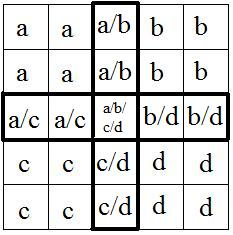
\includegraphics[width=0.5\linewidth]{Figures/kusquares}
  \caption{The Kuwahara Operator \cite{kuwahara_operator}}
  \label{fig:kusquares}
\end{figure}

Refer to Figure \ref{fig:LeeKu} for the resulting image.

\subsection{\label{sec:level2} Symmetric Nearest Neighbor (SNN) Filter}

The SNN filter is another sliding window filter that (like Kuwahara) aims to preserve edges, while decreasing noise. At every pixel the corners of the window are compared to the center pixel. The center pixel is the calculated mean sum of the selected pixels as shown in Figure \ref{fig:snn} \cite{fiveko_symmetric_2017}.

\begin{figure}
  \centering
  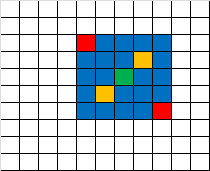
\includegraphics[width=0.5\linewidth]{Figures/snn}
  \caption{Symmetric Nearest Neighbor Pixel Selection \cite{fiveko_symmetric_2017}}
  \label{fig:snn}
\end{figure}

The Matlab implemenation by Art Barnes was chosen for applying this filter method to the OCT images \cite{barnes_snn_2005}. Refer to Figure \ref{fig:SNNhybrid} for the resulting image.
\subsection{\label{sec:level2} Hybrid Median Filter}
The Hybrid Median Filter is a nonlinear filter with better edge preseving characteristics than just an ordinary median filter. This is done by ranking spatial directions individually. This particular filter, filters matrix A using an $N \times N$ box. To apply the median filter three (3) medians are calculated in the $N \times N$ box. Where MR is the median of the horizontal and vertical R pixels, MD is the median of the diagonal D pixels. Using the 2 median and the central pixel value gives the filter value \cite{rabie_adaptive_2004}. For a $N=5$ matrix would give the following matrix:

$$
A =
\begin{bmatrix}
D & * & R & * & D\\
* & D & R & D & *\\
R & R & C & R & R\\
* & D & R & D & *\\
D & * & R & * & D\\
\end{bmatrix}
$$



The Matlab implementation by Damian Garcia was chosen for our analysis of this filter method on OCT images\cite{garcia_hybrid_2010}. The output image of this filter can be seen in Figure \ref{fig:SNNhybrid}.
\section{\label{sec:level1} Conclusion}
From the data gathered during the Matlab simulations, it is clear to see that image processing techniques greatly reduce noise and still have the ability to preserve edges. The calculated performance metrics used in matlab confirm this. Between the 5 different filters used the Wiener Filter performed the best in having a high Contrast to Noise Ratio (CNR) and Naturalness Image Quality Score (NIQE). This filter also produced a significantly lower Estimated Noise Level (ENL) as well. Refer to Table \ref{tab:compare} for the Matlab simulation quality metrics results. Although the Wiener filter performed the strongest using these quality metrics, the Hybrid Median filter and Lee filter would be more optimal for reducing speckle noise in OCT imagery. Both these filters have better edge preserving algorithms and still have quality CNR and NIQE scores.

\begin{table*}[]
  \begin{tabular}{|c|c|c|c|}
    \hline
    Filter Used & CNR & ENL & NIQE \\
    \hline
    No Filter & 9.0375 & 0.0247 & 10.823  \\
    \hline
    Wiener & 9.213 & 0.0077 & 5.95 \\
    \hline
    Lee & 8.316 & 0.0015 & 6.489 \\
    \hline
    Kuwahara & 8.878 & 0.0111 & 8.82 \\
    \hline
    Symmetric Neighbor & 8.788 & 0.0124 & 14.997\\
    \hline
    Hybrid Median  & 6.98 & 0.0069 & 7.817 \\
    \hline
  \end{tabular}
  \caption{Comparison of Filter Quality Metrics}
  \label{tab:compare}
\end{table*}

\begin{figure*}
  \centering
  \subfloat[Original Unfiltered Image]{\label{fig:unfilt}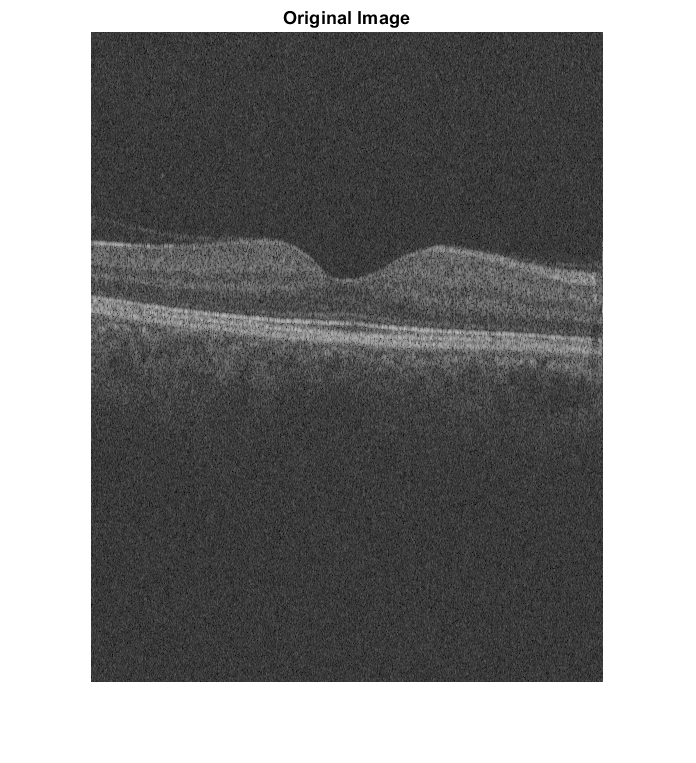
\includegraphics[width=0.5\textwidth]{Figures/orig}}
  \subfloat[Wiener Filtered Image]{\label{fig:wienerfilt}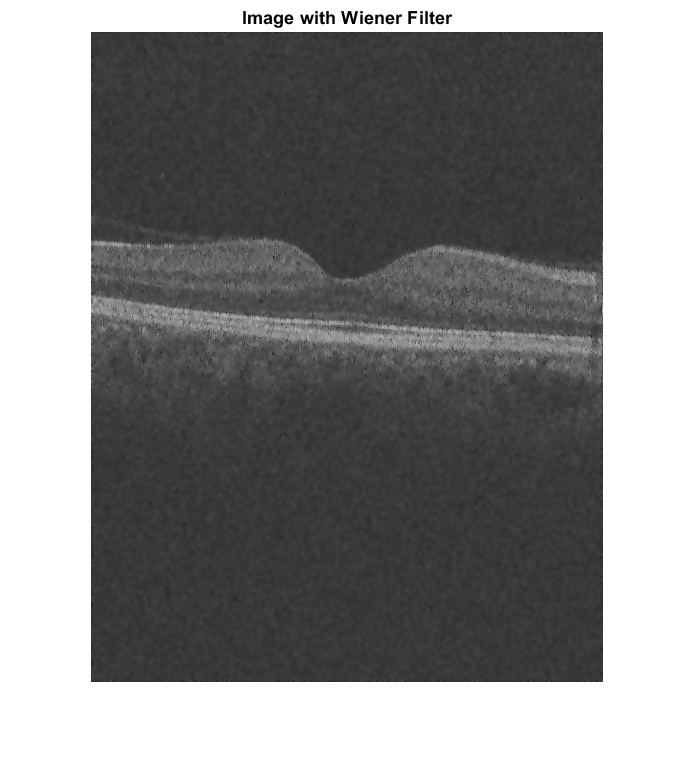
\includegraphics[width=0.5\textwidth]{Figures/wiener}}
  \caption{\label{fig:unfiltwienerfilt} Unfiltered and Wiener Filtered Images}
\end{figure*}

\begin{figure*}
  \centering
  \subfloat[Lee Filtered Image]{\label{fig:leefilt}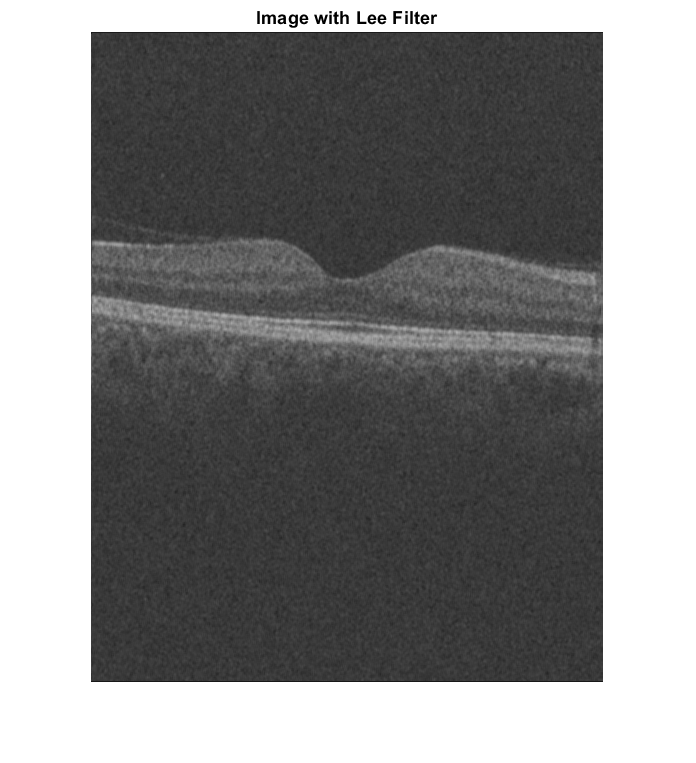
\includegraphics[width=0.5\textwidth]{Figures/lee}}
  \subfloat[Kuwahara Filtered Image]{\label{fig:kufilt}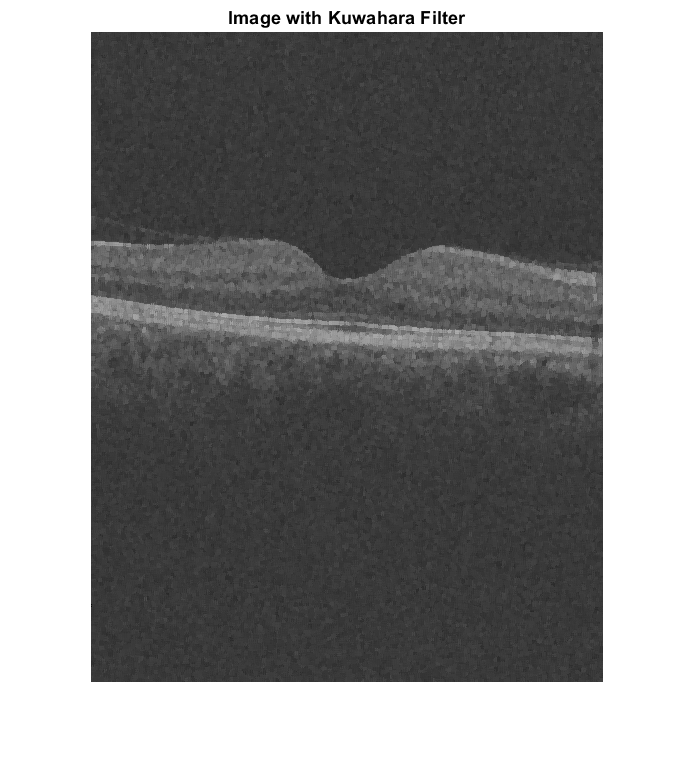
\includegraphics[width=0.5\textwidth]{Figures/Ku}}
  \caption{\label{fig:LeeKu} Lee and Kuwahara Filtered Images}
\end{figure*}

\begin{figure*}
  \centering
  \subfloat[SNN Filtered Image]{\label{fig:SNNfilt}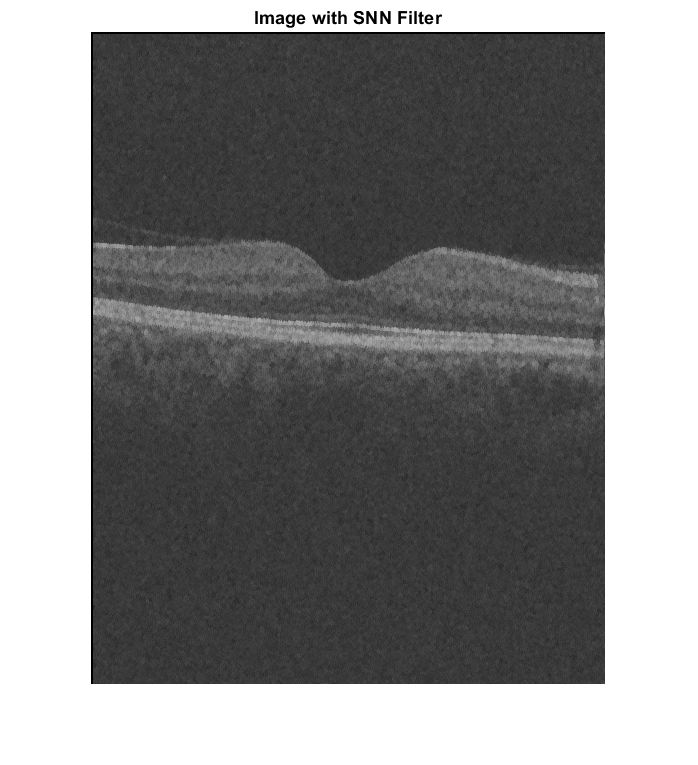
\includegraphics[width=0.5\textwidth]{Figures/SNNFilt}}
  \subfloat[Hyrbid Filtered Image]{\label{fig:hybridfilt}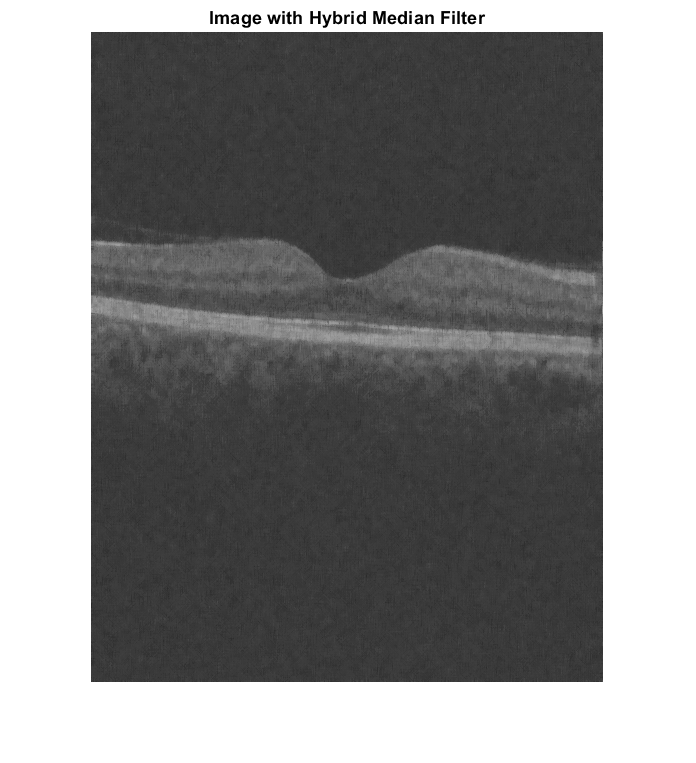
\includegraphics[width=0.5\textwidth]{Figures/hybrid}}
  \caption{\label{fig:SNNhybrid} SNN and Hybrid Filtered Images}
\end{figure*}
\clearpage
\noindent\begin{minipage}{.9\textwidth}
\begin{lstlisting}[language=Matlab, caption=Script to Generate Figure of Filtered Images and Print Quality Metrics, label=code:Allcoding]
  %Script to Open and Slice an OCT Image, Apply Filtering, and Print Quality Metrics

  clear all;
  close all;

  %Load and Slice 2D Image
  load('1_left.mat');
  img = mat2gray(d3(:,:,64), [0 255]);

  %Original Slice
  subplot (2,3,1), imshow(img)
  %figure, imshow(img)
  title('Original Image')

  %hybrid Median Filter
  M=hmf(img,9);
  subplot(2,3,3), imshow(M)
  %figure, imshow(M)
  title('Image with Hybrid Median Filter')
  [CNR,ENL,NIQESCORE] = EvaluateFilter(M);
  fprintf('\n CNR score HMF is %0.4f\n',CNR)
  fprintf('\n ENL score HMF is %0.4f\n',ENL)
  fprintf('\n NIQE score HMF is %0.4f\n',NIQESCORE)

  %Lee Filter
  [le]=lee1((d3(:,:,64)),1);
  subplot(2,3,4), imshow([le], [0 255])
  %figure, imshow([le], [0 255])
  title('Image with Lee Filter')
  [CNR,ENL,NIQESCORE] = EvaluateFilter([le]);
  fprintf('\n CNR score Lee is %0.4f\n',CNR)
  fprintf('\n ENL score Lee is %0.4f\n',ENL)
  fprintf('\n NIQE score Lee is %0.4f\n',NIQESCORE)

  %Symmetric Nearest Neighbor Filter
  H = snn(img,5,true);
  subplot(2,3,5), imshow(H)
  %figure, imshow(H)
  title('Image with SNN Filter')
  [CNR,ENL,NIQESCORE] = EvaluateFilter(H);
  fprintf('\n CNR score SNN is %0.4f\n',CNR)
  fprintf('\n ENL score SNN is %0.4f\n',ENL)
  fprintf('\n NIQE score SNN is %0.4f\n',NIQESCORE)

  %Kuwahara Filter
  filtered =Kuwahara(img,5);
  subplot(2,3,6), imshow(filtered)
  %figure, imshow(filtered)
  title('Image with Kuwahara Filter')
  [CNR,ENL,NIQESCORE] = EvaluateFilter(filtered);
  fprintf('\n CNR score Kuwahara is %0.4f\n',CNR)
  fprintf('\n ENL score Kuwahara is %0.4f\n',ENL)
  fprintf('\n NIQE score Kuwahara is %0.4f\n',NIQESCORE)

  %Wiener Filter
  K = wiener2(img,[5 5]);
  subplot(2,3,2), imshow(K)
  %figure, imshow(K)
  title('Image with Wiener Filter')
  [CNR,ENL,NIQESCORE] = EvaluateFilter(K);
  fprintf('\n CNR score Wiener is %0.4f\n',CNR)
  fprintf('\n ENL score Wiener is %0.4f\n',ENL)
  fprintf('\n NIQE score Wiener is %0.4f\n',NIQESCORE)
\end{lstlisting}
\end{minipage}

  \clearpage
	\bibliographystyle{apa}
	\bibliography{apssamp}% Produces the bibliography via BibTeX.
	\show\tableofcontents
	\show\lstlistoflistings
	\show\listoftables
	\show\listoffigures
\end{document}
%
% ****** End of file apssamp.tex ******
